\documentclass{standalone}
\usepackage{tikz}
\usetikzlibrary{patterns, positioning}
\usepackage[sfdefault]{ClearSans} %% option 'sfdefault' activates Clear Sans as the default text font
\usepackage[T1]{fontenc}

\begin{document}
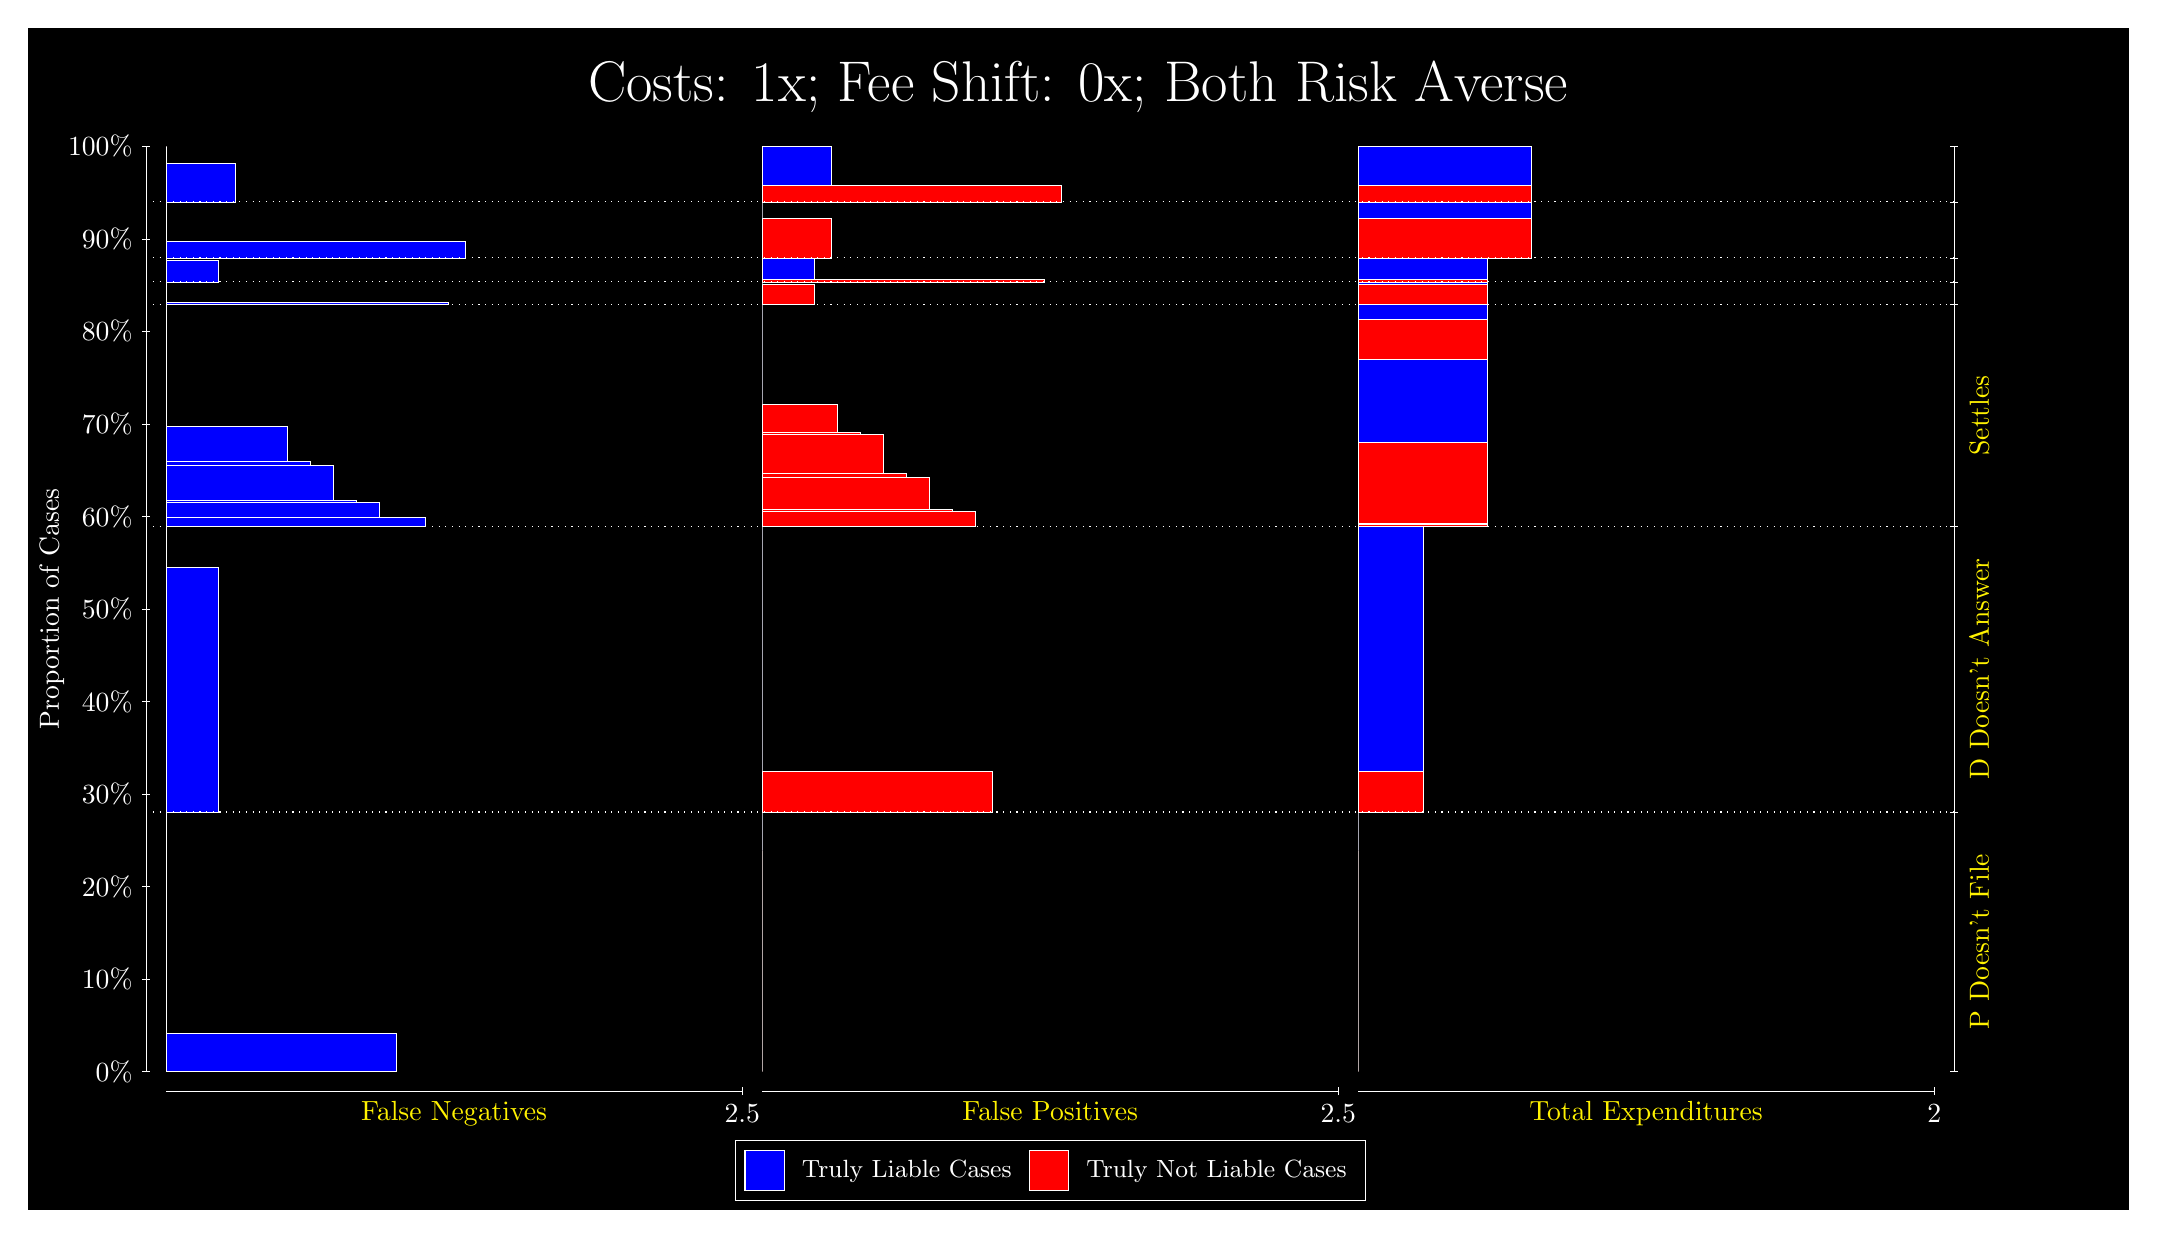
\begin{tikzpicture}
\draw[fill=black] (0,0) rectangle (26.667,15);
\draw[text=white] (0,13.5) rectangle (26.667,15) node[midway] {\huge Costs: 1x; Fee Shift: 0x; Both Risk Averse};
\draw[white, very thin] (1.5,1.75) -- (1.5,13.5);
\node[rotate=90, text=white, anchor=center] at (0.3, 7.625) {Proportion of Cases};
\draw[white, very thin] (1.45,1.75) -- (1.55,1.75);
\node[text=white, anchor=east] at (1.45, 1.75) {0\%};
\draw[white, very thin] (1.45,2.925) -- (1.55,2.925);
\node[text=white, anchor=east] at (1.45, 2.925) {10\%};
\draw[white, very thin] (1.45,4.1) -- (1.55,4.1);
\node[text=white, anchor=east] at (1.45, 4.1) {20\%};
\draw[white, very thin] (1.45,5.275) -- (1.55,5.275);
\node[text=white, anchor=east] at (1.45, 5.275) {30\%};
\draw[white, very thin] (1.45,6.45) -- (1.55,6.45);
\node[text=white, anchor=east] at (1.45, 6.45) {40\%};
\draw[white, very thin] (1.45,7.625) -- (1.55,7.625);
\node[text=white, anchor=east] at (1.45, 7.625) {50\%};
\draw[white, very thin] (1.45,8.8) -- (1.55,8.8);
\node[text=white, anchor=east] at (1.45, 8.8) {60\%};
\draw[white, very thin] (1.45,9.975) -- (1.55,9.975);
\node[text=white, anchor=east] at (1.45, 9.975) {70\%};
\draw[white, very thin] (1.45,11.15) -- (1.55,11.15);
\node[text=white, anchor=east] at (1.45, 11.15) {80\%};
\draw[white, very thin] (1.45,12.325) -- (1.55,12.325);
\node[text=white, anchor=east] at (1.45, 12.325) {90\%};
\draw[white, very thin] (1.45,13.5) -- (1.55,13.5);
\node[text=white, anchor=east] at (1.45, 13.5) {100\%};

\draw[white, very thin] (24.457,1.75) -- (24.457,13.5);
\draw[white, very thin] (24.407,1.75) -- (24.507,1.75);
\node[anchor=west] at (24.407, 1.75) {};
\draw[white, very thin] (24.407,5.0455) -- (24.507,5.0455);
\node[anchor=west] at (24.407, 5.0455) {};
\draw[white, very thin] (24.407,8.6768) -- (24.507,8.6768);
\node[anchor=west] at (24.407, 8.6768) {};
\draw[white, very thin] (24.407,11.488) -- (24.507,11.488);
\node[anchor=west] at (24.407, 11.488) {};
\draw[white, very thin] (24.407,11.779) -- (24.507,11.779);
\node[anchor=west] at (24.407, 11.779) {};
\draw[white, very thin] (24.407,12.084) -- (24.507,12.084);
\node[anchor=west] at (24.407, 12.084) {};
\draw[white, very thin] (24.407,12.794) -- (24.507,12.794);
\node[anchor=west] at (24.407, 12.794) {};
\draw[white, very thin] (24.407,13.5) -- (24.507,13.5);
\node[anchor=west] at (24.407, 13.5) {};

\draw[white, very thin, fill=blue] (1.75,1.75) rectangle (4.6775,2.236);
\draw[white, very thin, fill=red] (1.75,2.236) rectangle (1.75,5.0455);
\draw[white, very thin, fill=blue] (1.75,5.0455) rectangle (2.4087,8.1587);
\draw[white, very thin, fill=red] (1.75,8.1587) rectangle (1.75,8.6768);
\draw[white, very thin, fill=blue] (1.75,8.6768) rectangle (5.0435,8.7831);
\draw[white, very thin, fill=blue] (1.75,8.7831) rectangle (4.7507,8.7879);
\draw[white, very thin, fill=blue] (1.75,8.7879) rectangle (4.458,8.978);
\draw[white, very thin, fill=blue] (1.75,8.978) rectangle (4.1652,9.0069);
\draw[white, very thin, fill=blue] (1.75,9.0069) rectangle (3.8725,9.4432);
\draw[white, very thin, fill=blue] (1.75,9.4432) rectangle (3.5797,9.4995);
\draw[white, very thin, fill=blue] (1.75,9.4995) rectangle (3.287,9.9427);
\draw[white, very thin, fill=red] (1.75,9.9427) rectangle (1.75,11.488);
\draw[white, very thin, fill=blue] (1.75,11.488) rectangle (5.3362,11.518);
\draw[white, very thin, fill=red] (1.75,11.518) rectangle (1.75,11.779);
\draw[white, very thin, fill=blue] (1.75,11.779) rectangle (2.4087,12.052);
\draw[white, very thin, fill=red] (1.75,12.052) rectangle (1.75,12.084);
\draw[white, very thin, fill=blue] (1.75,12.084) rectangle (5.5558,12.294);
\draw[white, very thin, fill=red] (1.75,12.294) rectangle (1.75,12.794);
\draw[white, very thin, fill=blue] (1.75,12.794) rectangle (2.6283,13.29);
\draw[white, very thin, fill=red] (1.75,13.29) rectangle (1.75,13.5);
\draw[white, very thin, fill=red] (9.3189,1.75) rectangle (9.3189,4.5595);
\draw[white, very thin, fill=blue] (9.3189,4.5595) rectangle (9.3189,5.0455);
\draw[white, very thin, fill=red] (9.3189,5.0455) rectangle (12.246,5.5636);
\draw[white, very thin, fill=blue] (9.3189,5.5636) rectangle (9.3189,8.6768);
\draw[white, very thin, fill=red] (9.3189,8.6768) rectangle (12.027,8.8635);
\draw[white, very thin, fill=red] (9.3189,8.8635) rectangle (11.734,8.8898);
\draw[white, very thin, fill=red] (9.3189,8.8898) rectangle (11.441,9.2907);
\draw[white, very thin, fill=red] (9.3189,9.2907) rectangle (11.149,9.3458);
\draw[white, very thin, fill=red] (9.3189,9.3458) rectangle (10.856,9.844);
\draw[white, very thin, fill=red] (9.3189,9.844) rectangle (10.563,9.8669);
\draw[white, very thin, fill=red] (9.3189,9.8669) rectangle (10.27,10.222);
\draw[white, very thin, fill=blue] (9.3189,10.222) rectangle (9.3189,11.488);
\draw[white, very thin, fill=red] (9.3189,11.488) rectangle (9.9776,11.748);
\draw[white, very thin, fill=blue] (9.3189,11.748) rectangle (9.3189,11.779);
\draw[white, very thin, fill=red] (9.3189,11.779) rectangle (12.905,11.811);
\draw[white, very thin, fill=blue] (9.3189,11.811) rectangle (9.9776,12.084);
\draw[white, very thin, fill=red] (9.3189,12.084) rectangle (10.197,12.584);
\draw[white, very thin, fill=blue] (9.3189,12.584) rectangle (9.3189,12.794);
\draw[white, very thin, fill=red] (9.3189,12.794) rectangle (13.125,13.003);
\draw[white, very thin, fill=blue] (9.3189,13.003) rectangle (10.197,13.5);
\draw[white, very thin, fill=red] (16.888,1.75) rectangle (16.888,4.5595);
\draw[white, very thin, fill=blue] (16.888,4.5595) rectangle (16.888,5.0455);
\draw[white, very thin, fill=red] (16.888,5.0455) rectangle (17.711,5.5636);
\draw[white, very thin, fill=blue] (16.888,5.5636) rectangle (17.711,8.6768);
\draw[white, very thin, fill=red] (16.888,8.6768) rectangle (18.534,8.6956);
\draw[white, very thin, fill=blue] (16.888,8.6956) rectangle (18.534,8.7073);
\draw[white, very thin, fill=red] (16.888,8.7073) rectangle (18.534,9.7353);
\draw[white, very thin, fill=blue] (16.888,9.7353) rectangle (18.534,10.799);
\draw[white, very thin, fill=red] (16.888,10.799) rectangle (18.534,11.298);
\draw[white, very thin, fill=blue] (16.888,11.298) rectangle (18.534,11.488);
\draw[white, very thin, fill=red] (16.888,11.488) rectangle (18.534,11.748);
\draw[white, very thin, fill=blue] (16.888,11.748) rectangle (18.534,11.779);
\draw[white, very thin, fill=red] (16.888,11.779) rectangle (18.534,11.811);
\draw[white, very thin, fill=blue] (16.888,11.811) rectangle (18.534,12.084);
\draw[white, very thin, fill=red] (16.888,12.084) rectangle (19.083,12.584);
\draw[white, very thin, fill=blue] (16.888,12.584) rectangle (19.083,12.794);
\draw[white, very thin, fill=red] (16.888,12.794) rectangle (19.083,13.003);
\draw[white, very thin, fill=blue] (16.888,13.003) rectangle (19.083,13.5);
\draw[white, dotted] (1.5,5.0455) -- (24.457,5.0455);
\draw[white, dotted] (1.5,8.6768) -- (24.457,8.6768);
\draw[white, dotted] (1.5,11.488) -- (24.457,11.488);
\draw[white, dotted] (1.5,11.779) -- (24.457,11.779);
\draw[white, dotted] (1.5,12.084) -- (24.457,12.084);
\draw[white, dotted] (1.5,12.794) -- (24.457,12.794);
\draw[white, very thin] (1.75,1.5) -- (9.0689,1.5);
\node[text=yellow, anchor=north] at (5.4094, 1.5) {False Negatives};
\draw[white, very thin] (9.0689,1.45) -- (9.0689,1.55);
\node[text=white, anchor=north] at (9.0689, 1.45) {2.5};

\draw[white, very thin] (9.3189,1.5) -- (16.638,1.5);
\node[text=yellow, anchor=north] at (12.978, 1.5) {False Positives};
\draw[white, very thin] (16.638,1.45) -- (16.638,1.55);
\node[text=white, anchor=north] at (16.638, 1.45) {2.5};

\draw[white, very thin] (16.888,1.5) -- (24.207,1.5);
\node[text=yellow, anchor=north] at (20.547, 1.5) {Total Expenditures};
\draw[white, very thin] (24.207,1.45) -- (24.207,1.55);
\node[text=white, anchor=north] at (24.207, 1.45) {2};

\node[text=yellow, centered, rotate=90] at (24.777, 3.3977) {P Doesn't File};
\node[text=yellow, centered, rotate=90] at (24.777, 6.8611) {D Doesn't Answer};
\node[text=yellow, centered, rotate=90] at (24.777, 10.082) {Settles};





\draw (12.978300999999998,1.5) node[draw=none] (baseCoordinate) {};
\begin{scope}[align=center]
        \matrix[scale=0.5, draw=white, below=0.5cm of baseCoordinate, nodes={draw}, column sep=0.1cm]{
            \node[rectangle, draw, minimum width=0.5cm, minimum height=0.5cm, fill=blue] {}; &
            \node[draw=none, font=\small, text=white] (B) {Truly Liable Cases}; &
            \node[rectangle, draw, minimum width=0.5cm, minimum height=0.5cm, fill=red] {}; &
            \node[draw=none, font=\small, text=white] (B) {Truly Not Liable Cases}; \\
            };
\end{scope}

\end{tikzpicture}
\end{document}